%!TEX root = PMP_ClockPendulumAnalyzer.tex
\section{Test}
Dieses Kapitel erläutert das Testen des \documenttitle.
	\subsection{Testumgebung}
    In diesem Kapitel ist die ganze Testumgebung erläutert, damit exakte und nachvollziehbare Tests gemacht werden können.
    \subsubsection{Aufstellung}
    Der Pendulum Analyzer wird mittels einer normalen Wand-Pendeluhr getestet. Dazu wird die Uhr in einer dafür hergestellten Verschalung aufgehängt (abgebildet in Bild \ref{fig:verschalung}).
    \begin{figure}[H]
        \centering
        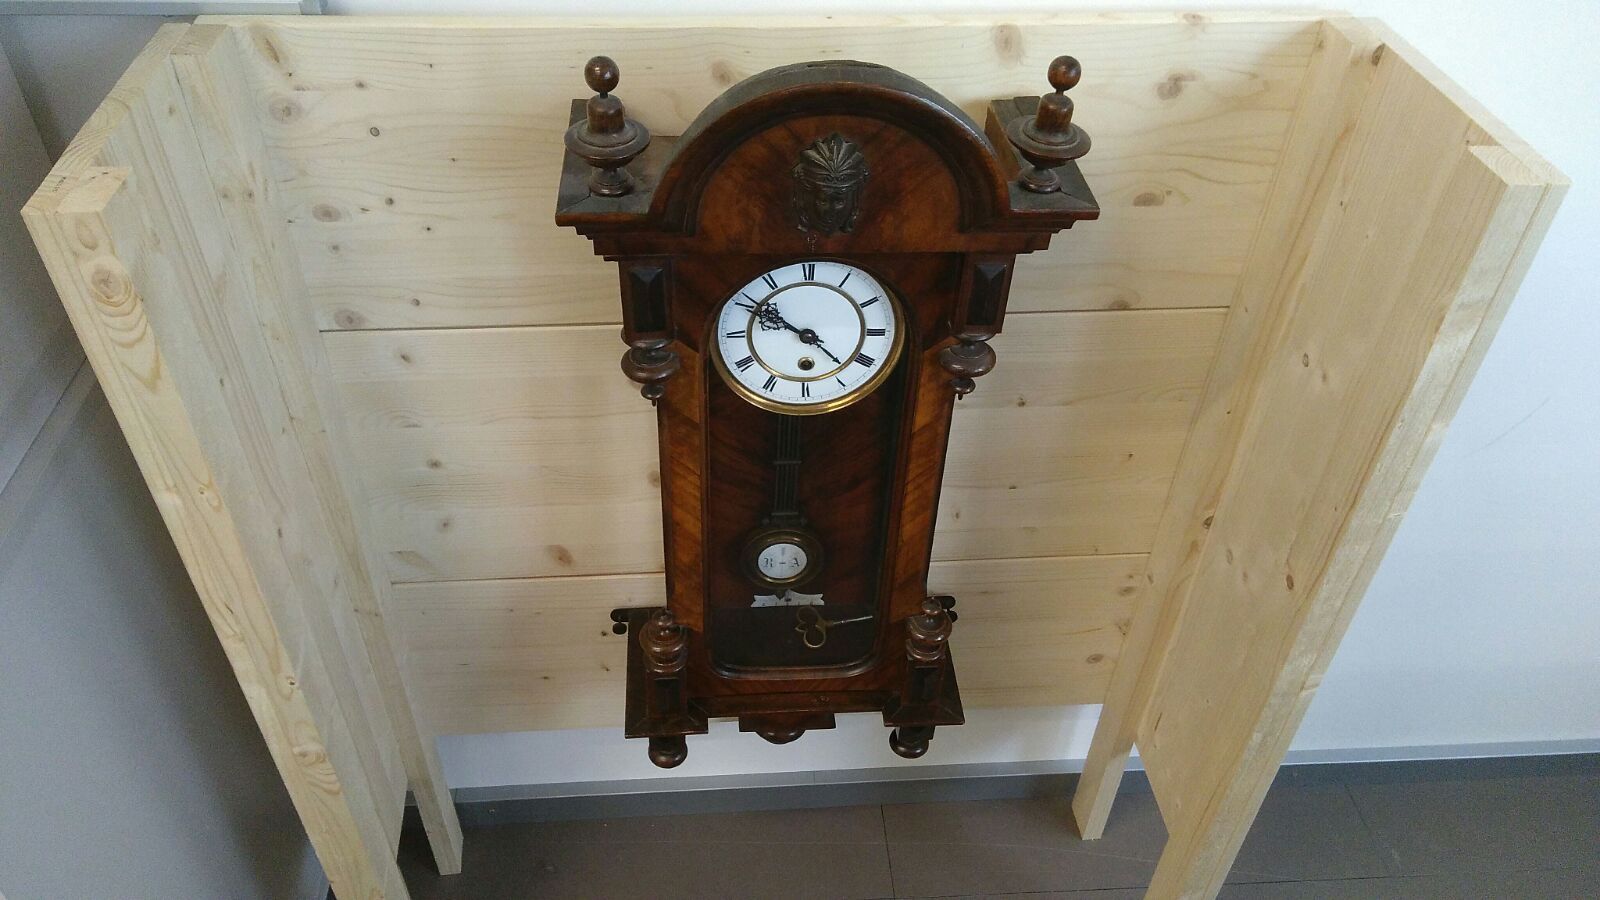
\includegraphics[width=.5\textwidth]{verschalung_neu.png}
        \caption{Verschalung für die Pendeluhr}
        \label{fig:verschalung}
    \end{figure}

    \noindent Die Uhr hat eine Fläche auf der die Sensoraufhängung platziert werden kann.
    Die restlichen Systemteile können unterhalb der Uhr auf dem Boden platziert werden (siehe Abbildung \ref{fig:uhrboden}).
    \begin{figure}[h]
        \centering
        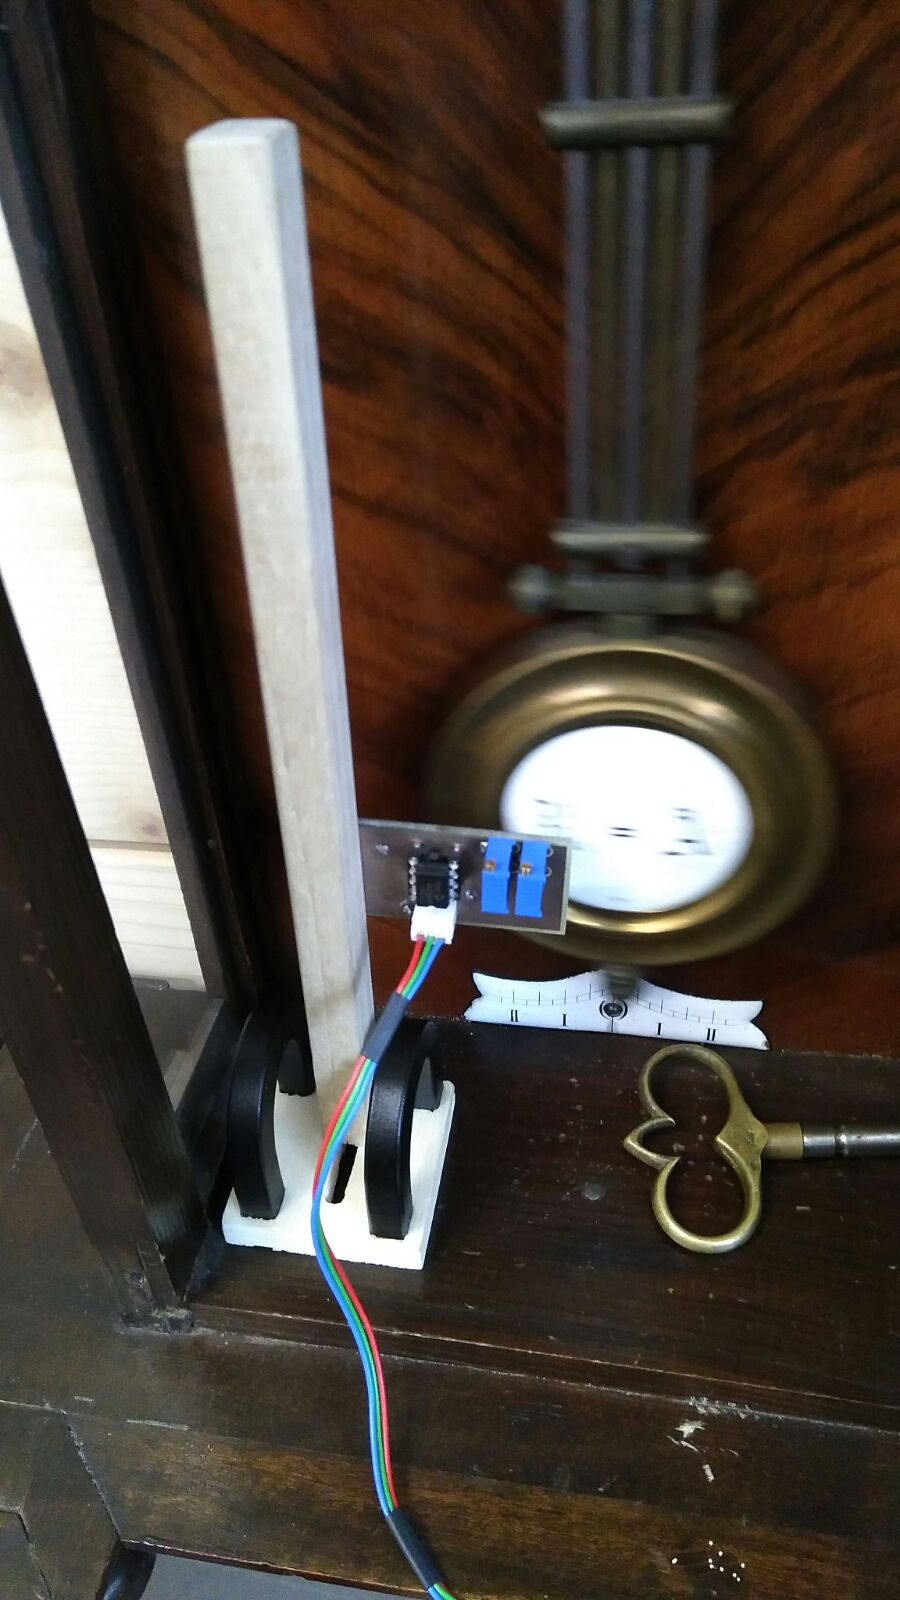
\includegraphics[width=.3\textwidth]{sensor_aufstellung.png}
        \caption{Sensoraufhängung auf dem Uhrenboden}
        \label{fig:uhrboden}
    \end{figure}
    
    \clearpage
    \subsubsection{Sensor Montage}
    Es wird mit nur einem Sensor gearbeitet.
    Dieser wird an einer einfachen Holzstange montiert.
    Die Höhe ist über 17 Positionen verstellbar und stufenlos in der Länge. Im Bild \ref{fig:sensor_montage} ist der Stab zu sehen, an welchem der Sensor montiert wird.
    \begin{figure}[H]
        \centering
        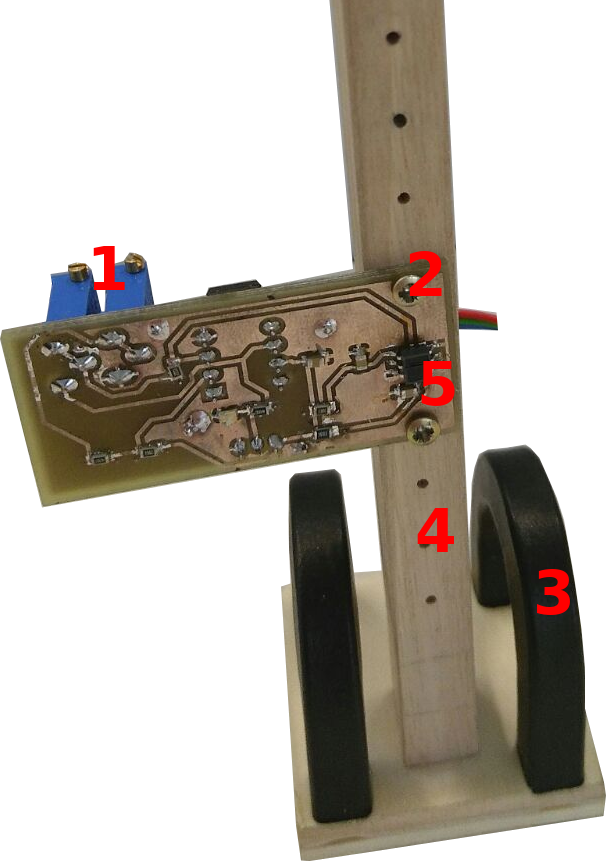
\includegraphics[width=.5\textwidth]{sensor_aufhangung_neu.png}
        \caption{Stab zur Sensormontage mit Sensorboard}
        \label{fig:sensor_montage}
    \end{figure}
    \begin{enumerate}
        \item Potentiometer für das Justieren des Sensors
        \item Schraube zum montieren
        \item Gewicht zur Stabilisierung
        \item Vorbohrungen zur Höhenverstellung
        \item Sensor
    \end{enumerate}

    \clearpage
    \subsection{Testfälle}
    Dieses Kapitel beschreibt Testfälle welche manuell ausgeführt werden, um eine korrekte Funktionalität zu gewährleisten.
    	\subsubsection{Integrations-Tests}
            %\newcommand{\tempitem}{\labelitemi}
\renewcommand{\labelitemi}{-}

\begin{table}[H]
	\begin{tabularx}{\textwidth}{ | p{0.22\textwidth} | p{0.68\textwidth} |} \hline
		\rowcolor{gray!50}
		%Titelzeile
			\textbf{ID} & \textbf{I1}\\ \hline
		%Zeile
			\textbf{Bezeichnung} & 
            Ermitteln Referenzfrequenz ohne GPS Verbindung.\\ \hline
		%Zeile
			\textbf{Beschreibung} & 
            Die Referenzfrequenz wird mittels FIX-Pin des GPS-Moduls ermittelt.\\ \hline
		%Zeile
			\textbf{Akteure} &
            Entwickler\\ \hline
		%Zeile
			\textbf{Vorbedingungen} &
            \begin{itemize}
                \item USB-Verbindung von \hwb\ zu einem Test-PC oder Notebook.
                \item Optische Überprüfung des laufenden \hwb.
                \item Die FIX-LED des GPS-Moduls auf dem \hwb\ blinkt im Sekundentakt.
                \item Konsolenprogramm zum Empfang von UART-RS232 Signalen gestartet.
            \end{itemize}\\ \hline
		%Zeile
			\textbf{Ergebnis} &        
			\begin{itemize}
				\item Die Referenzfrequenzen werden jede Sekunde aufgelistet.
				\item Die Streuung zwischen den Werten entspricht der Streuung gemäss Systemspezifikation (Kapitel ).
			\end{itemize}\\ \hline
		%Zeile
			\textbf{Ergebnis bei Fehler} &
			\begin{itemize}
				\item Fehlerhafte oder fehlende Werte in der Anzeige.
				\item Anzeigen auf dem \hwb\ verhalten sich nicht erwartungsgemäss.
			\end{itemize}\\ \hline
		%Zeile
			\textbf{Ablauf} &
			\begin{enumerate}
				\item USB-Verbindung erstellen.
				\item Terminal-Programm starten (z.B. Minicom)
				\item Ergebnis prüfen
			\end{enumerate}\\ \hline
        %Zeile
			\textbf{Testdaten} &
            Keine benötigt.\\ \hline
        %Untere Abgrenzung
	\end{tabularx}
	\caption{Integrationstest 1}
	\label{tab:inttest1}
\end{table}

\renewcommand{\labelitemi}{$\bullet$}

        \clearpage
    	%\subsubsection{System-Tests}